% Simplified attribution graph visualisation
% Depicts transcoder feature nodes across layers with attribution edges
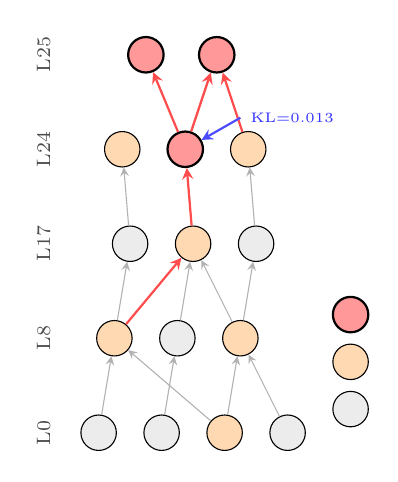
\begin{tikzpicture}[
  node distance=0.6cm and 1.2cm,
  feat/.style={circle, draw, minimum size=0.45cm, inner sep=0pt, font=\tiny},
  high/.style={feat, fill=red!40, thick},
  med/.style={feat, fill=orange!30},
  low/.style={feat, fill=gray!15},
  edge/.style={->, >=stealth, thin, gray!60},
  strong/.style={->, >=stealth, thick, red!70},
  label/.style={font=\scriptsize, text=black!70},
]

% Layer labels
\node[label, rotate=90] at (-0.7, 0) {L0};
\node[label, rotate=90] at (-0.7, 1.2) {L8};
\node[label, rotate=90] at (-0.7, 2.4) {L17};
\node[label, rotate=90] at (-0.7, 3.6) {L24};
\node[label, rotate=90] at (-0.7, 4.8) {L25};

% Layer 0 features
\node[low] (f00) at (0, 0) {};
\node[low] (f01) at (0.8, 0) {};
\node[med] (f02) at (1.6, 0) {};
\node[low] (f03) at (2.4, 0) {};

% Layer 8 features
\node[med] (f10) at (0.2, 1.2) {};
\node[low] (f11) at (1.0, 1.2) {};
\node[med] (f12) at (1.8, 1.2) {};

% Layer 17 features
\node[low] (f20) at (0.4, 2.4) {};
\node[med] (f21) at (1.2, 2.4) {};
\node[low] (f22) at (2.0, 2.4) {};

% Layer 24 features
\node[med] (f30) at (0.3, 3.6) {};
\node[high] (f31) at (1.1, 3.6) {};
\node[med] (f32) at (1.9, 3.6) {};

% Layer 25 features (output)
\node[high] (f40) at (0.6, 4.8) {};
\node[high] (f41) at (1.5, 4.8) {};

% Attribution edges (weak)
\draw[edge] (f00) -- (f10);
\draw[edge] (f01) -- (f11);
\draw[edge] (f02) -- (f10);
\draw[edge] (f02) -- (f12);
\draw[edge] (f03) -- (f12);
\draw[edge] (f10) -- (f20);
\draw[edge] (f11) -- (f21);
\draw[edge] (f12) -- (f21);
\draw[edge] (f12) -- (f22);
\draw[edge] (f20) -- (f30);
\draw[edge] (f22) -- (f32);

% Strong attribution edges (high causal influence)
\draw[strong] (f10) -- (f21);
\draw[strong] (f21) -- (f31);
\draw[strong] (f31) -- (f40);
\draw[strong] (f31) -- (f41);
\draw[strong] (f32) -- (f41);

% Legend
\node[low, label=right:{\scriptsize Low importance}] at (3.2, 0.3) {};
\node[med, label=right:{\scriptsize Moderate}] at (3.2, 0.9) {};
\node[high, label=right:{\scriptsize High importance}] at (3.2, 1.5) {};

% Annotation
\draw[<-, >=stealth, thick, blue!70] (f31) -- ++(0.7, 0.4) node[right, font=\tiny, text=blue!80] {KL=0.013};
\end{tikzpicture}
